%----------------------------------------------------------------------------
% Magic tutorial number 9
%----------------------------------------------------------------------------

\NeedsTeXFormat{LaTeX2e}[1994/12/01]
\documentclass[letterpaper,twoside,12pt]{article}
\usepackage{epsfig,times}

\setlength{\textwidth}{8.5in}
\addtolength{\textwidth}{-2.0in}
\setlength{\textheight}{11.0in}
\addtolength{\textheight}{-2.0in}
\setlength{\oddsidemargin}{0in}
\setlength{\evensidemargin}{0pt}
\setlength{\topmargin}{-0.5in}
\setlength{\headheight}{0.2in}
\setlength{\headsep}{0.3in}
\setlength{\topskip}{0pt}

\def\hinch{\hspace*{0.5in}}
\def\starti{\begin{center}\begin{tabbing}\hinch\=\hinch\=\hinch\=hinch\hinch\=\kill}
\def\endi{\end{tabbing}\end{center}}
\def\ii{\>\>\>}
\def\mytitle{Magic Tutorial \#9: Format Conversion for CIF and Calma}

%----------------------------------------------------------------------------

\begin{document}

\makeatletter
\newcommand{\ps@magic}{%
	\renewcommand{\@oddhead}{\mytitle\hfil\today}%
	\renewcommand{\@evenhead}{\today\hfil\mytitle}%
	\renewcommand{\@evenfoot}{\hfil\textrm{--{\thepage}--}\hfil}%
	\renewcommand{\@oddfoot}{\@evenfoot}}
\newcommand{\ps@mplain}{%
	\renewcommand{\@oddhead}{}%
	\renewcommand{\@evenhead}{}%
	\renewcommand{\@evenfoot}{\hfil\textrm{--{\thepage}--}\hfil}%
	\renewcommand{\@oddfoot}{\@evenfoot}}
\makeatother
\pagestyle{magic}
\thispagestyle{mplain}


\begin{center}
  {\bfseries \Large \mytitle} \\
  \vspace*{0.5in}
  {\itshape John Ousterhout} \\
  \vspace*{0.5in}
   Computer Science Division \\
   Electrical Engineering and Computer Sciences \\
   University of California \\
   Berkeley, CA  94720 \\
  \vspace*{0.25in}
  {\itshape (Updated by others, too.)} \\
  \vspace*{0.25in}
  This tutorial corresponds to Magic version 7. \\
\end{center}
\vspace*{0.5in}

{\noindent\bfseries\large Tutorials to read first:}
\starti
   \> Magic Tutorial \#1: Getting Started \\
   \> Magic Tutorial \#2: Basic Painting and Selection \\
   \> Magic Tutorial \#4: Cell Hierarchies
\endi

{\noindent\bfseries\large Commands introduced in this tutorial:}
\starti
   \> :calma, :cif
\endi

{\noindent\bfseries\large Macros introduced in this tutorial:}

\starti
   \> {\itshape (None)}
\endi

\vspace*{0.75in}
\section{Basics}

CIF (Caltech Intermediate Form) and Calma Stream Format are
standard layout description languages used to transfer mask-level layouts
between organizations and design tools.  This tutorial describes
how Magic can be used to read and write files in CIF and Stream
formats.  The version of CIF that Magic supports is CIF 2.0; it
is the most popular layout language in the university design
community.  The Calma format that Magic supports is GDS II Stream
format, version 3.0, corresponding to GDS II Release 5.1.  This
is probably the most popular layout description language for the
industrial design community.

To write out a CIF file, place the cursor over a layout window
and type the command

\starti
   \ii {\bfseries :cif}
\endi

This will generate a CIF file called {\itshape name}{\bfseries .cif}, where
{\itshape name} is the name of the root cell in the window.  The CIF
file will contain a description of the entire cell
hierarchy in that window.  If you wish to use a name different
from the root cell, type the command

\starti
   \ii {\bfseries :cif write} {\itshape file}
\endi

This will store the CIF in {\itshape file}{\bfseries .cif}.  Start Magic up
to edit {\bfseries tut9a} and
generate CIF for that cell.  The CIF file
will be in ASCII format, so you can use Unix commands
like {\bfseries more} and {\bfseries vi} to see what it contains.

To read a CIF file into Magic, place the cursor over a layout window
and type the command

\starti
   \ii {\bfseries :cif read} {\itshape file}
\endi

This will read the file {\itshape file}{\bfseries .cif} (which must be in
CIF format), generate Magic cells for the hierarchy described
in the file, make the entire hierarchy a subcell of the
edit cell, and run the design-rule checker to verify everything
read from the file.  Information in the top-level cell (usually
just a call on the ``main'' cell of the layout) will be placed
into the edit cell.  Start Magic up afresh and read in {\bfseries tut9a.cif},
which you created above.  It will be easier if you always read
CIF when Magic has just been started up:  if some of the cells
already exist, the CIF reader will not overwrite them, but will
instead use numbers for cell names.

To read and write Stream-format files, use the commands
{\bfseries :calma read} and {\bfseries :calma}, respectively.  These commands
have the same effect as the CIF commands, except that they
operate on files with {\bfseries .strm} extensions.  Stream is a binary
format, so you can't examine {\bfseries .strm} files with a text editor.

Stream files do not identify a top-level cell, so you won't see
anything on the screen after you've used the {\bfseries :calma read}
command.  You'll have to use the {\bfseries :load} command to look at
the cells you read.  However, if Magic was used to write the
Calma file being read, the library name reported by the
{\bfseries :calma read} command is the same as the name of the
root cell for that library.

Also, Calma format places some limitations on the names of cells:
they can only contain alphanumeric characters, ``\$'', and ``{\_}'',
and can be at most 32 characters long.  If the name of a cell does
not meet these limitations, {\bfseries :calma write} converts it to a
unique name of the form \rule{0.25in}{0.5pt}{\itshape n}, where
{\itshape n} is a small
integer.  To avoid any possible conflicts, you should avoid using
names like these for your own cells.

You shouldn't need to know much more than what's above in order
to read and write CIF and Stream.  The sections below describe the different
styles of CIF/Calma that Magic can generate and the limitations
of the CIF/Calma facilities (you may have noticed that when you
wrote and read CIF above you didn't quite get back what you started
with;  Section 3 describes the differences that can occur).
Although the discussion mentions
only CIF, the same features and problems apply to Calma.

\section{Styles}

Magic usually knows several different ways to generate
CIF/Calma from a given layout.  Each of these ways is called a {\itshape style}.
Different styles can be used to handle different
fabrication facilities, which may differ in the names they use for
layers or in the exact mask set required for fabrication.
Different styles can be also used to write out CIF/Calma with slightly
different feature sizes or design rules.  CIF/Calma
styles are described in the technology file that Magic reads when
it starts up;  the exact number and nature of the styles is
determined by whoever wrote your technology file.  There are separate
styles for reading and writing CIF/Calma;  at any given time, there
is one current input style and one current output style.

The standard SCMOS technology file provides an example of how
different styles can be used.  Start up Magic with the
SCMOS technology ({\bfseries magic -Tscmos}).  Then type the commands

\starti
   \ii {\bfseries :cif ostyle} \\
   \ii {\bfseries :cif istyle}
\endi

The first command will print out a list of all the styles in
which Magic can write CIF/Calma (in this technology) and the second
command prints out the styles in which Magic can read CIF/Calma.
You use the {\bfseries :cif} command to change the current styles, but
the styles are used for both CIF and Calma format conversion.
The SCMOS technology file provides several output styles.
The initial (default) style for writing CIF is {\bfseries lambda=1.0(gen)}.
This style generates mask layers for the MOSIS scalable
CMOS process, where each Magic unit corresponds to 1 micron and
both well polarities are generated.  See the technology manual
for more information on the various styles that are available.
You can change the output style with the command

\starti
   \ii {\bfseries :cif ostyle} {\itshape newStyle}
\endi

where {\itshape newStyle} is the new style you'd like to use for output.
After this command, any future CIF or Calma files will be generated
with the new style.  The {\bfseries :cif istyle} command can be used
in the same way to see the available styles for reading CIF and
to change the current style.

Each style has a specific scalefactor;  you can't use a
particular style with a different scalefactor.  To change
the scalefactor, you'll have to edit the appropriate
style in the {\bfseries cifinput} or {\bfseries cifoutput} section
of the technology file.  This process is described in
``Magic Maintainer's Manual \#2: The Technology
File.''

\section{Rounding}

The units used for coordinates in Magic are generally different
from those in CIF files.  In Magic, most technology files use
lambda-based units, where one unit is typically half the minimum
feature size.  In CIF files, the units are centimicrons (hundredths
of a micron).  When
reading CIF and Calma files, an integer scalefactor is used to
convert from centimicrons to Magic units.  If the CIF file contains
coordinates that don't scale exactly to integer Magic units,
Magic rounds the coordinates up or down to the closest integer
Magic units.  A CIF coordinate exactly halfway between two Magic
units is rounded down.  The final authority on rounding is the
procedure CIFScaleCoord in the file cif/CIFreadutils.c
When rounding occurs, the resulting Magic file will
not match the CIF file exactly.

Technology files usually specify geometrical operations such as
bloating, shrinking, and-ing, and or-ing to be performed on
CIF geometries when they are read into Magic.  These geometrical
operations are all performed in the CIF coordinate system (centimicrons)
so there is no rounding or loss of accuracy in the operations.
Rounding occurs only AFTER the geometrical operations, at the last
possible instant before entering paint into the Magic database.

\section{Non-Manhattan Geometries}

Magic only supports Manhattan features.  When CIF or Calma files
contain non-Manhattan features, they are approximated with
Manhattan ones.  The approximations occur for wires (if the
centerline contains non-Manhattan segments) and polygons
(if the outline contains non-Manhattan segments).  In
these cases, the non-Manhattan segments are replaced with one
or more horizontal and vertical segments before the figure is
processed.  Conversion is done by inserting a one-unit stairstep
on a 45-degree angle until a point is reached where a horizontal
or vertical line can reach the segment's endpoint.  Some
examples are illustrated in the figure below:  in each case, the
figure on the left is the one specified in the CIF file, and the
figure on the right is what results in Magic.

\begin{figure}[ht]
   \begin{center}
      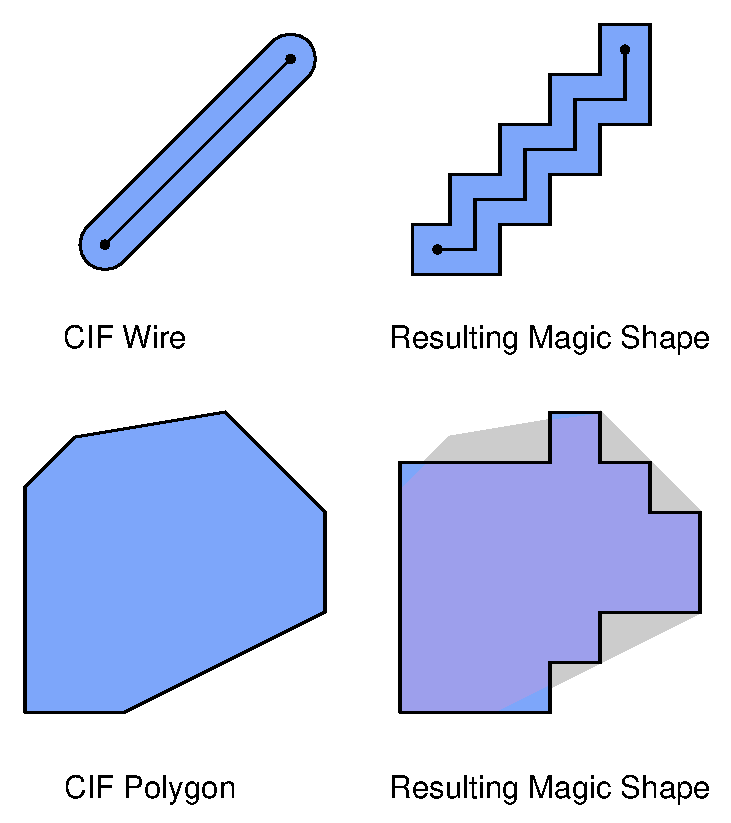
\epsfig{file=../psfigures/tut9.1.ps, width=0.55\columnwidth}
   \end{center}
\end{figure}

The shape of the Magic stairstep depends on the order in which
vertices appear in the CIF or Calma file.  The stairstep is made
by first incrementing or decrementing the x-coordinate, then
incrementing or decrementing the y-coordinate, then x, then y,
and so on.  For example, in the figure above, the polygon was
specified in counter-clockwise order;  if it had been specified
in clockwise order the result would have been slightly different.

An additional approximation occurs for wires.  The CIF wire figure
assumes that round caps will be generated at each end of the wire.
In Magic, square caps are generated instead.  The top example
of the figure above illustrates this approximation.


\section{Other Problems with Reading and Writing CIF}

You may have noticed that when you wrote out CIF for {\bfseries tut9a}
and read it back in again, you didn't get back quite what you
started with.  Although the differences shouldn't cause any serious
problems, this section describes what they are so you'll know what
to expect.  There are three areas where there may be discrepancies:
labels, arrays, and contacts.  These are illustrated in {\bfseries tut9b}.
Load this cell, then generate CIF, then read the CIF
back in again.  When the CIF is read in, you'll get a couple of
warning messages because Magic won't allow the CIF to overwrite
existing cells:  it uses new numbered cells instead (this is
why you should normally read CIF with a ``clean slate'';  in
this case it's convenient to have both the original and
reconstructed infromation present at the same time;  just
ignore the warnings). The information
from the CIF cell appears as a subcell named {\bfseries 1} right on
top of the old contents of {\bfseries tut9b};  select {\bfseries 1},
move it below {\bfseries tut9b}, and expand it so you can compare
its contents to {\bfseries tut9b}.

The first problem area is that CIF normally allows only point labels.  By
default, where you have line or box labels in Magic,
CIF labels are generated at the center of the Magic labels.
The label {\bfseries in} in {\bfseries tut9y} is an example of a line label
that gets smashed in the CIF processing.  The command

\starti
   \ii {\bfseries :cif arealabels yes}
\endi

sets a switch telling Magic to use an extension to cif to output 
area-labels.  This is not the default since many programs that
take CIF as input do not understand this extension.

If you are reading a CIF file created by a tool other than Magic,
there is an additional problems with labels.  The CIF label construct
(``{\bfseries 94} {\itshape label x y layer}'') has an optional {\itshape layer} field
that indicates the layer to which a label is attached.  If reading
a CIF file generated by Magic, this field is always present and so
a label's layer is unambiguous.  However, if the field is absent,
Magic must decide which layer to use.  It does this by looking to
see what Magic layers lie beneath the label after the CIF has been
read in.  When there are several layers, it chooses the one appearing
LATEST in the {\bfseries types} section of the technology file.  Usually,
it's possible to ensure that the right layer is used by placing
signal layers (such as metal, diffusion, and poly) later in the
types section than layers such as pwell or nplus.  However, sometimes
Magic will still pick the wrong layer, and it will be up to you to
move the label to the right layer yourself.

The second problem is with arrays.  CIF has no standard array
construct, so when Magic outputs arrays it does it as a collection
of cell instances.  When the CIF file is read back in, each array
element comes back as a separate subcell.
The array of {\bfseries tut9y} cells is an example of this.
Most designs only have
a few arrays that are large enough to matter;  where this is the
case, you should go back after reading the CIF and replace the
multiple instances with a single array.
Calma format does have an array construct, so it
doesn't have this problem.

The third discrepancy is that where there are large contact areas,
when CIF is read and written the area of the contact may be
reduced slightly.  This happened to the large poly contact in
{\bfseries tut9b}.  The shrink doesn't reduce the effective area of
the contact;  it just reduces the area drawn in Magic.
To see what's happening here, place
the box around {\bfseries tut9b} and {\bfseries 1}, expand everything,
then type

\starti
   \ii {\bfseries :cif see CCP}
\endi

This causes feedback to be displayed showing CIF layer ``CCP''
(contact cut to poly).  You may have to zoom in a bit to
distinguish the individual via holes.  Magic generates lots of
small contact vias over
the area of the contact, and if contacts aren't exact multiples
of the hole size and spacing then extra space is left around
the edges.  When the CIF is read back in, this extra space isn't
turned back into contact.  The circuit that is read in is
functionally identical to the original circuit, even though
the Magic contact appears slightly smaller.

There is an additional problem with generating CIF having to
do with the cell hierarchy.  When Magic generates CIF, it performs
geometric operations such as ``grow'' and ``shrink''on the mask
layers.  Some of these operations are not guaranteed to work
perfectly on hierarchical designs.  Magic detects when there are
problems and creates feedback areas to mark the trouble spots.
When you write CIF, Magic will warn you that there were troubles.
These should almost never happen if you generate CIF from designs
that don't have any design-rule errors.  If they do occur, you
can get around them by writing cif with the following command

\starti
   \ii {\bfseries :cif flat} {\itshape fileName}
\endi

This command creates an internal version of the design with hierarchy
removed, before outputing CIF as in {\bfseries cif write}.  An alternative
approach that does not require flattening is to modify the technology
file in use.  Read ``Magic Maintainers Manual \#2:  The Technology File'',
if you want to try this approach.

\end{document}
